% Kugelmodell des Armplaners als 3D-Ansicht (orthografisch), linke Hand, gleicher Maßstab in a) und b).
% Eigene Darstellung, Renderings aus dem G1-Code (siehe Daten/kugelmodell/README.md).
\begin{tikzpicture}[ba]
  \node[anchor=north west, inner sep=0] (A) at (0,0) {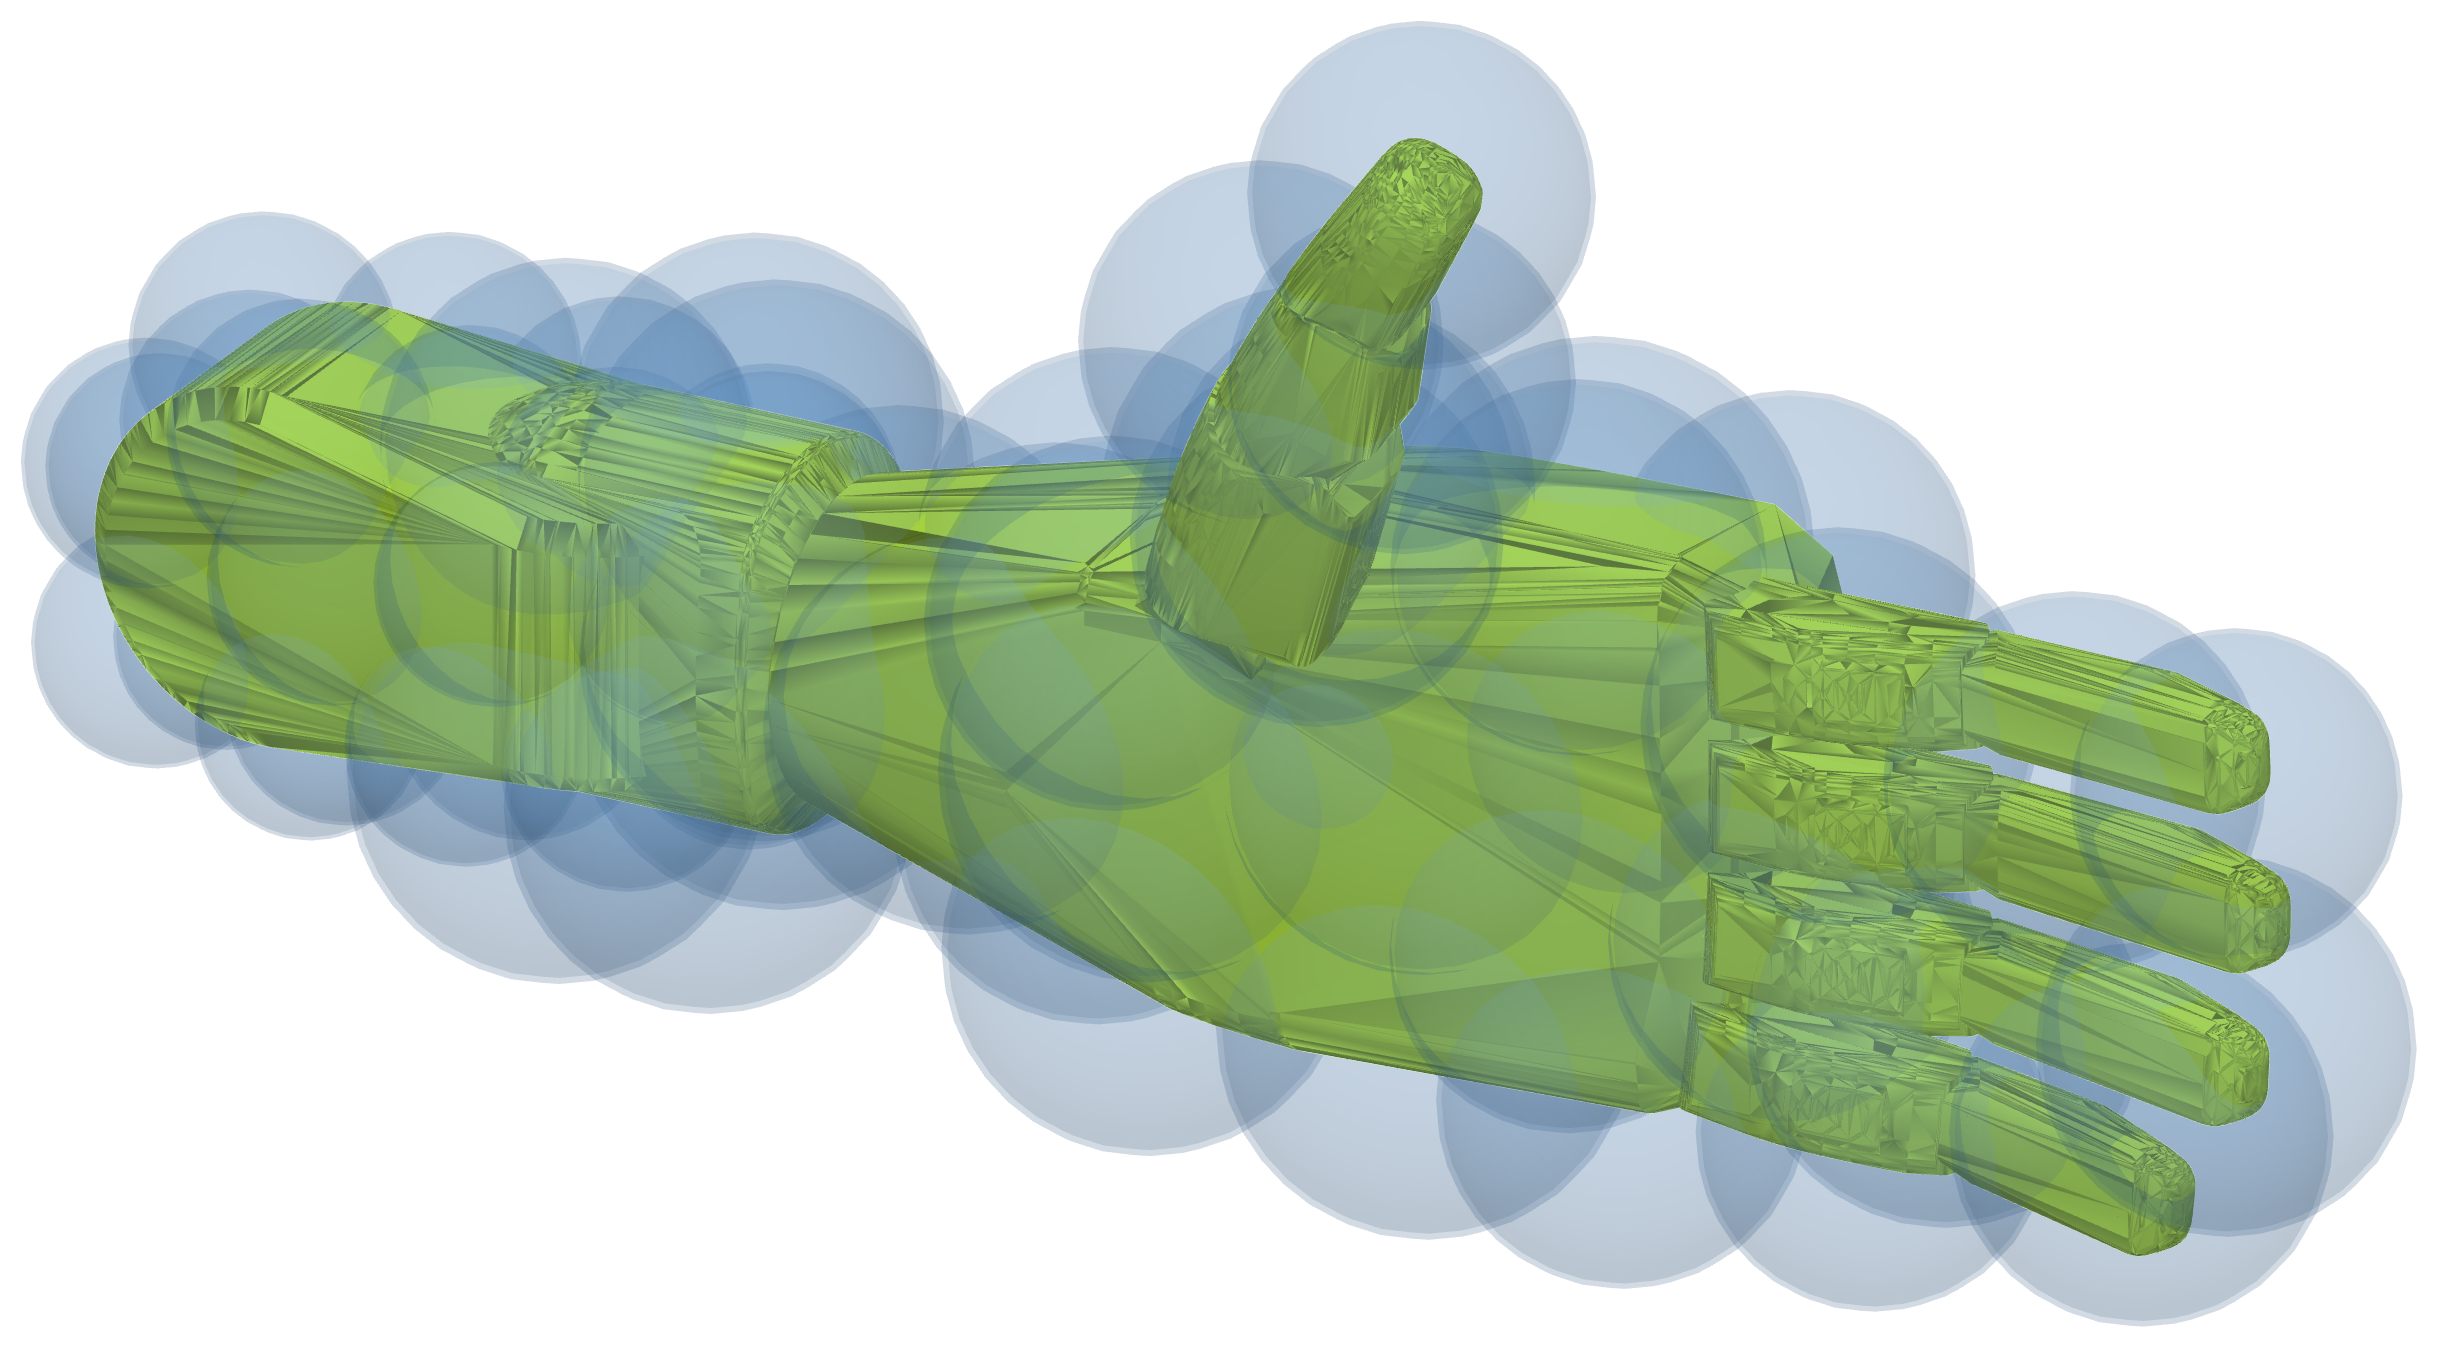
\includegraphics[width=14cm]{Bilder/kugelmodell-3d-inspire.png}};
  \node[ba teiltitel, anchor=north west] at ($(A.south west)+(0,-0.1)$) {a) Inspire-Hand (Modell auch für die Rubber Hand verwendet)};
  \node[anchor=north west, inner sep=0] (B) at ($(A.south west)+(0,-0.9)$) {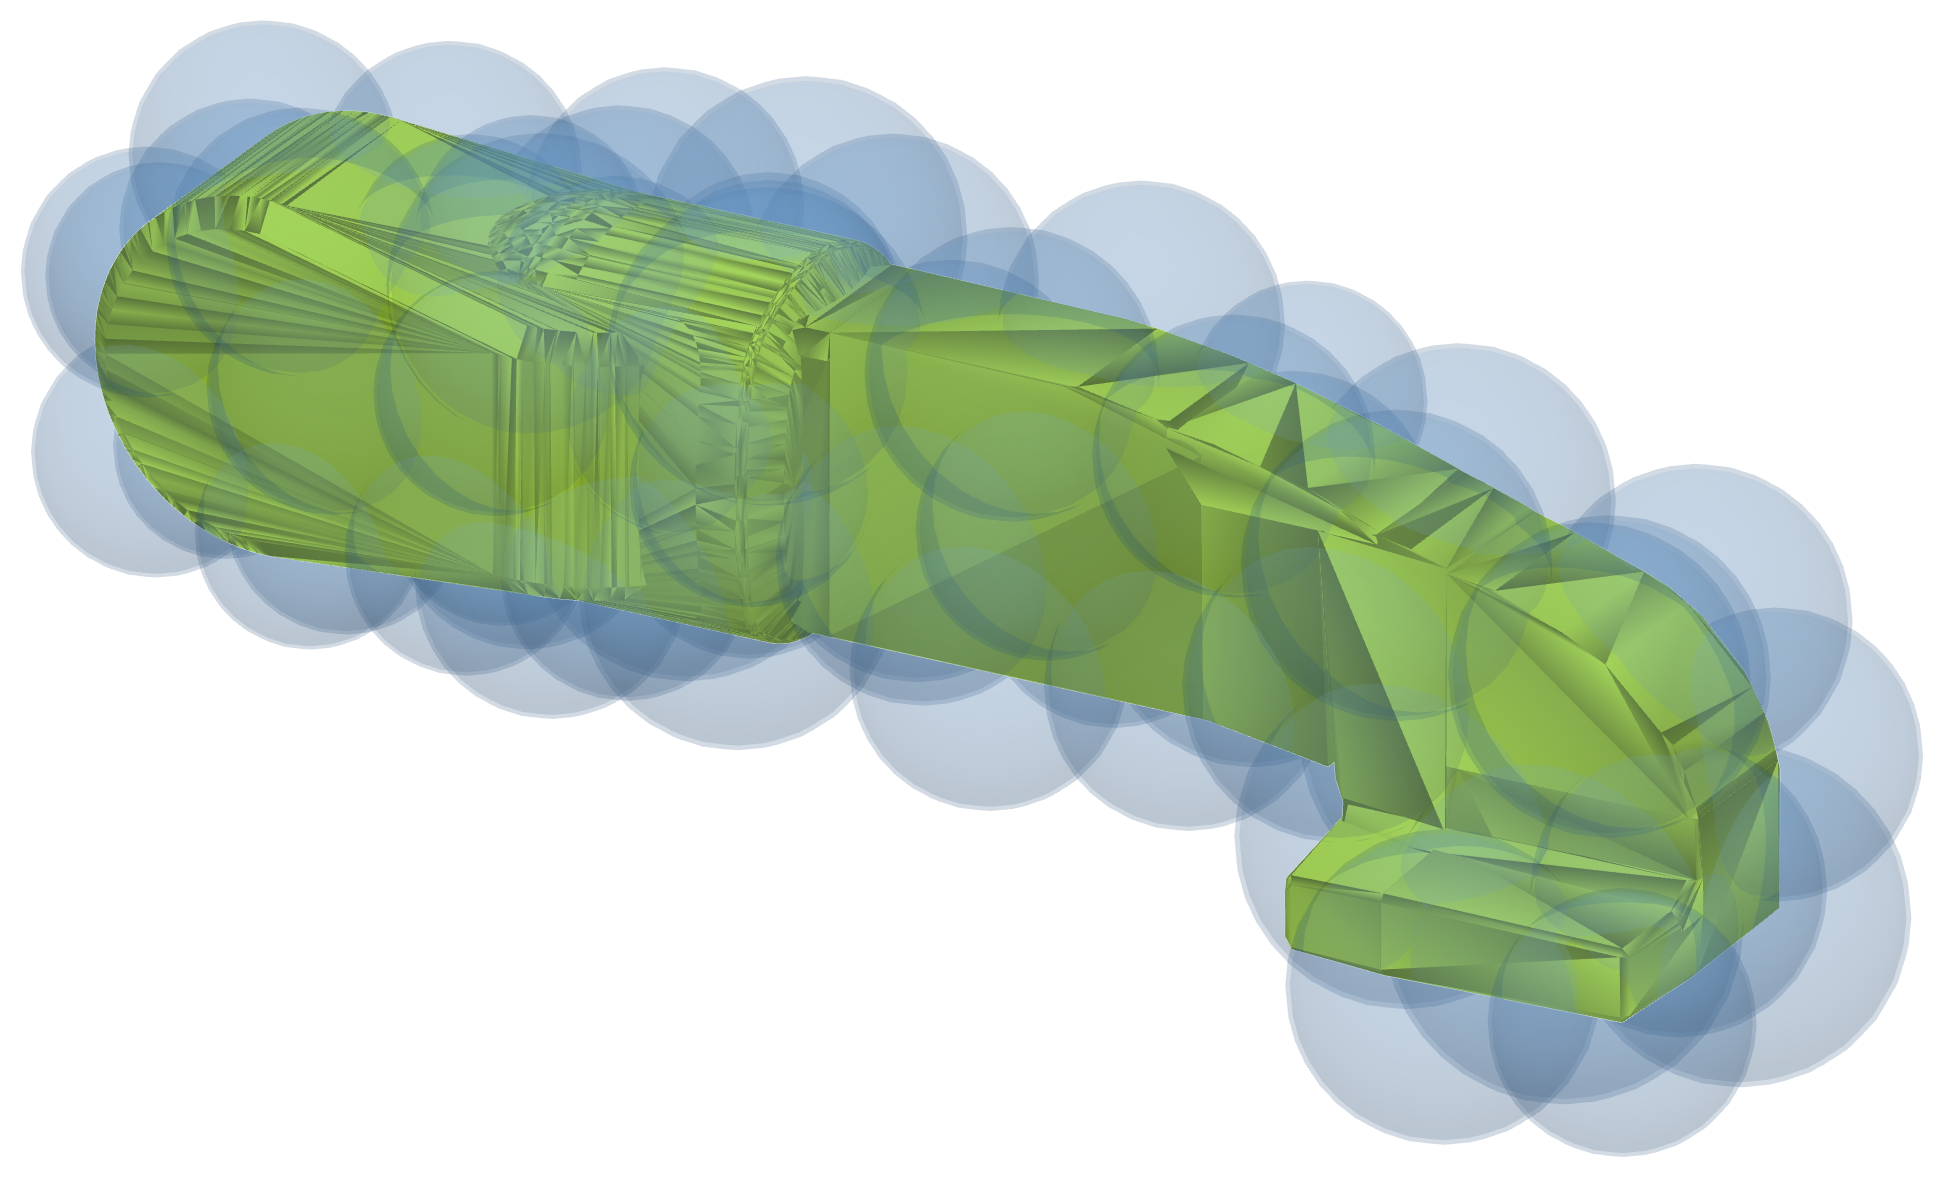
\includegraphics[width=11.16cm]{Bilder/kugelmodell-3d-haken.png}};
  \node[ba teiltitel, anchor=north west] at ($(B.south west)+(0,-0.1)$) {b) Gedruckter Box-Haken (Hand-Profil)};
  \fill[baGruen, draw=baGruen] ($(B.south west)+(0,-1.0)$) rectangle ++(0.4,0.3);
  \node[anchor=west] at ($(B.south west)+(0.45,-0.85)$) {Kollisionsgeometrie};
  \fill[baHellblau, fill opacity=0.45, draw=baBlau, draw opacity=0.5] ($(B.south west)+(4.4,-0.85)$) circle (0.17);
  \node[anchor=west] at ($(B.south west)+(4.65,-0.85)$) {Kugel des Planers};
\end{tikzpicture}
